\documentclass[class=NCU_thesis, crop=false]{standalone}
\begin{document}

\chapter{實驗背景與動機}
\section{古典通訊展頻}
展頻技術 (Spread Spectrum Technology) 在古典通訊上已行之有年,最初為軍事或情報單位訊號傳遞使用,以避避免電波干擾或訊號攔截,現今此技術以廣泛運用無無線電通訊中。

根據 FCC(Federal Communications Committee;美國聯邦通訊委員會)規定的 ISM(Industrial Scientific, and Medical),在特定頻段內不需申請執照及可供民間、工業、科學與醫學用途使用,由於任何設備可自由使用這些頻段來傳遞訊息,這些頻段上會十分擁擠,訊號可能會互相影響,如\cref{fig:jamming},而使用展頻技術即可解決此頻段共享的問題。一般而言展頻技術主要可分成跳頻展頻(Frequency Hopping Spread Spectrum, FHSS)和直接序列展頻(Direct Sequence Spread Spectrum, DSSS),以下簡單介紹這兩者的原理與應用。


\fig[0.5][fig:jamming][!htb]{jamming.png}[同頻訊號干擾。發送端發出之訊號,紅色為其他訊號源發出之同頻訊號干擾。][同頻訊號干擾]

藍芽技術上,使用的頻段為 2.4 GHz,在 ISM 規範的波段內,會與無線電話、無線網路等設備共享頻段,若同時有兩個以上訊號使用同樣的頻率來傳輸,由於接收端無法區分訊號的來源,會相互干擾,想克服此問題可使用跳頻技術:傳輸端每秒改變訊號的頻率數次,接收端以對應的頻率去接收訊號,示意圖\cref{fig:fhss},如此可避免特定頻段遭占用的問題。

\begin{figure}[!hbt]
    %\captionsetup[subfigure]{labelformat=empty} % 完全隱藏圖號
    \centering
    \subcaptionbox
        {Channel assignment
        \label{fig:fhss_channel_assignment}}
        {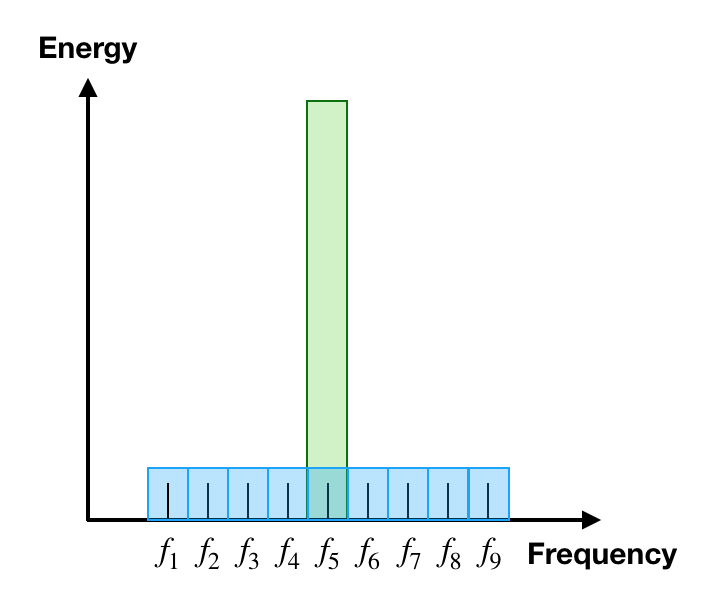
\includegraphics[width=0.4\linewidth]{fhss_channel_assignment.png}}
    ~~~~
    \subcaptionbox
        {Chaneel use
        \label{fig:fhss_channel_use}}
        {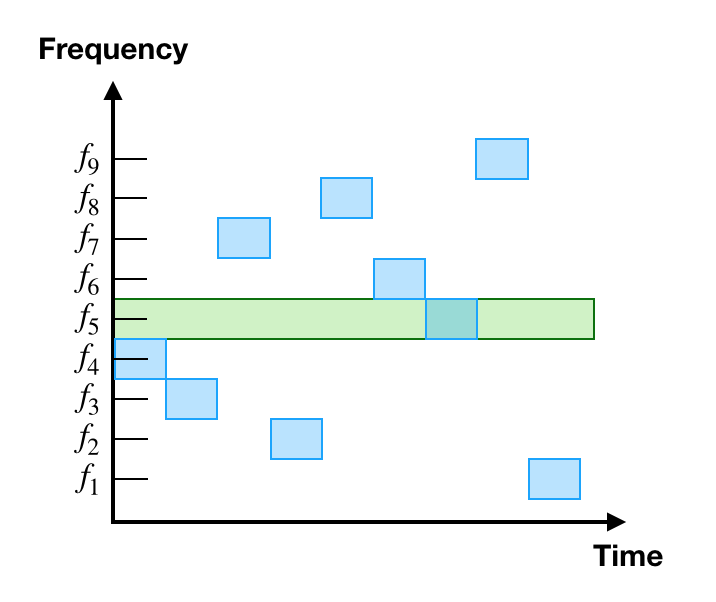
\includegraphics[width=0.4\linewidth]{fhss_channel_use.png}}
    \caption{跳頻展頻技術示意圖,綠色為展頻前,藍色為展頻後。\cref{fig:fhss_channel_assignment} 為指定的頻率分佈,展頻前僅使用 $f_5$ 這個頻率通道進行傳輸,展頻後則將訊號分成數個頻率,不同時間以不同頻率進行傳輸,如\cref{fig:fhss_channel_use}}
    \label{fig:fhss}
\end{figure}

直接序列展頻技術則是以一串特定的高頻訊號,對發動端的原始資訊進行調製,將頻譜展寬,如\cref{fig:dsss_spread},接收端再以相同的高頻訊號對其進行解碼,還原出原始的資訊。此種方式可以有效的降低同頻訊號的干擾,示意圖如\cref{fig:dsss}。DSSS 提供一種穩定且簡單的解決方案,能以低功率高頻寬遠距傳輸資訊,廣泛應用於無線網路、無線電話、GPRS...等,但相較於跳頻展頻技術,直接序列展頻技術需要較高的硬體建置成本。

\fig[0.5][fig:dsss_spread][!htb]{dsss_spread.png}[直接序列展頻技術,對原始訊號進行調製且展寬其頻寬。]

\begin{figure}[!hbt]
    %\captionsetup[subfigure]{labelformat=empty} % 完全隱藏圖號
    \centering
    \subcaptionbox
        {展頻後傳輸訊號
        \label{fig:dsss_spread_jamming}}
        {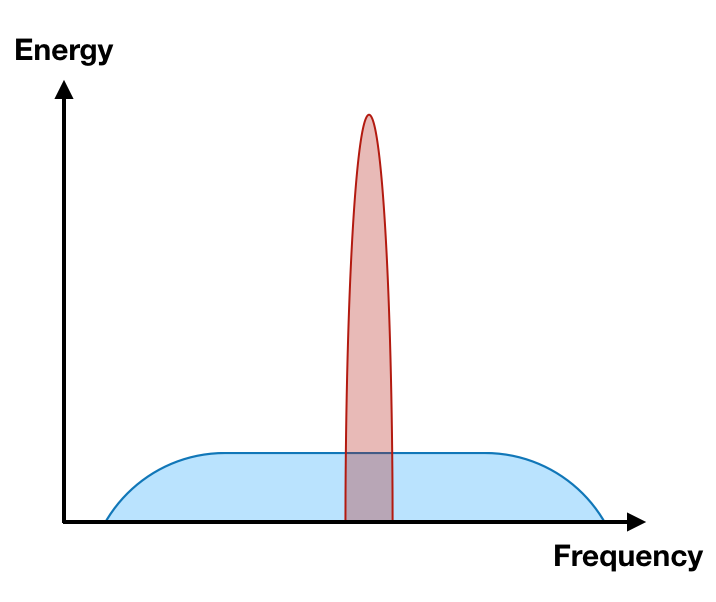
\includegraphics[width=0.4\linewidth]{dsss_spread_jamming.png}}
    ~~~~
    \subcaptionbox
        {解展頻後接收訊號
        \label{fig:dsss_compress_jamming}}
        {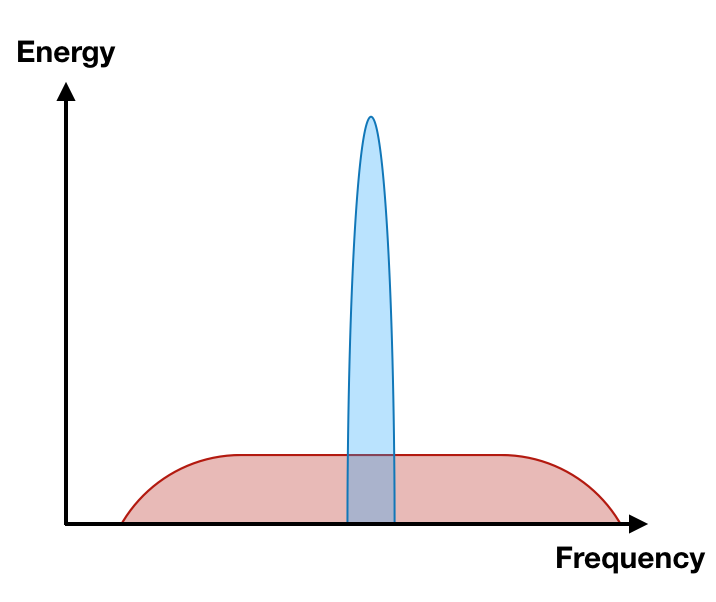
\includegraphics[width=0.4\linewidth]{dsss_compress_jamming.png}}
    \caption{直接序列展頻技術示意圖。\cref{fig:dsss_spread_jamming} 藍色為已展頻之發送端訊號,紅色為同頻訊號干擾。\cref{fig:dsss_compress_jamming} 為接收端解展頻後的訊號,藍色訊號被回復成原始的狀態,紅色的同頻訊號則被展頻,能量被打散至各個不同的頻率,可降低接收端的收到的雜訊。}
    \label{fig:dsss}
\end{figure}


\section{量子通訊展頻}
在量子資訊中,有許多的應用都要以單光子作為攜帶資訊的媒介,以量子密鑰分發而言,各種加密協定如 BB84, DPS-QKD 提供了傳輸密鑰的方式,但卻無法確保訊號能在不被干擾的情況下抵達接受端,所以若能將展頻技術應用在單光子上,降低環境或人為干擾對遠距傳輸的影響,則可提升資料傳輸的效率與安全性。

\section{研究介紹}
基於上述之實驗背景與動機,我們研究的目的為將展頻技術運用於單光子上,在第二章中會介紹展頻的原理,從數學的角度去探究相位調製對頻譜的影響;第三章中會以前一章的數學原理,以我們的實驗的條件進行模擬,並計算當光子與原子產生交互作用下時的頻譜變化;第四章介紹實驗上會用到的重要儀器;第五章介紹實驗的流程並討論實驗結果,最後再針對實際測量到的結果對理論進行修正與比較。

\end{document}